 
\documentclass[french]{article}
 
\usepackage[utf8]{inputenc}
\usepackage[T1]{fontenc}
\usepackage{babel}
 
 \usepackage{hyperref}
\hypersetup{
    colorlinks=true,
    linkcolor=blue,
    filecolor=magenta,      
    urlcolor=cyan,
}
 
\urlstyle{same}

\usepackage{graphicx}

\title{Devoir de programmaction PC2R - Scrabble}
\author{Sofiane GHERSA}
\date{2017} 
 
\begin{document}


\maketitle

\includegraphics{images/logo_upmc.png}
 
\tableofcontents

\vspace{2cm} %Add a 2cm space
 
\begin{abstract}
    Réaliser d'une application clients-serveur permettant
a des utilisateurs de jouer a un jeu de lettre multijoueurs (type Scrabble Duplicate ).
\end{abstract}
 
\section{ But Du devoir}
    On fournit a tous les participants connectes l’état du plateau de jeu (des cases
éventuellement remplies de lettres) et le même tirage de 7 lettres; les participants envoient
des propositions de placement des lettres sur le plateau.

\noindent
\setlength { \parindent } {5ex }
    a la fin du tour, tous les participants marquent des points en fonction de leur
placement et le jeu continue pour tous les participants avec le plateau obtenu après le
meilleur placement propos.
 
\noindent
\setlength { \parindent } {5ex }
    On envoi le meilleur mot avec son score et celui qui la trouve et le scores de toute les
joueur a chaque tour et le numéro de ce tour grâce a \textbf{BILAN/mot/vainqueur/scores/}   
\noindent scores : n*user1*score1*user2*score2*…
\noindent je considère que « user1 » le nom de joueur qui reçois et « score1 » c’est son score .

\section{Langage utilise }
    Le langage JAVA pour le cote Serveur : je le trouve mieux pour les thread et la
gestion de la concurrence.

\noindent
\setlength { \parindent } {5ex }
        Le langage C pour le cote Client : grâce a la bibliothèque GLADE qui nous facilite le
travaille sur les interface graphique et elle donne la possibilité de traiter les événement soit
en C ou PYTHON .

\section{ Réglés du jeu}
    les même règle que le \href{https://www-apr.lip6.fr/~chaillou/Public/enseignement/2016-2017/pc2r/public/projet-16-3.pdf}{Sujet}  vous trouve en bas les changement qu’on a fait dans les
deux cote . 
 
\section{Protocole} 
    le dictionnaire : on utilise GLAFF , on a fait quelque modification sur le dictionnaire
( on a sépare les mots dans plusieurs fichier en fonction de sa première lettre EX : le fichier
« A\_dico.txt » il contienne tout les mots qui commence par ‘A’ on a fait ça pour facilite
l'accès et la vérification des mots ) .

\noindent
\setlength { \parindent } {5ex }
    le serveur écoute sur le port 2017 en TCP . On peux garder les valeurs compte-arebours
qu’on a sur le sujet ou initialiser notre propre valeur .

\noindent
\setlength { \parindent } {5ex }
    Les commande on utilise celle de sujet juste qu’on a ignore \textbf{VAINQUEUR/bilan/}
on utilise que \textbf{BILAN/mot/vainqueur/scores/} même a la fin de session .

\section{ SERVEUR }
\subsection{ Tirage }
    On pioche aléatoirement les lettre dans notre réservoir a la fin de tour si aucun na
trouve un mot on pioche 7 nouvelle lettre sinon on garde celle qui ne son pas utilise et on
pioche les autre , si le nombre de lettre qui reste dans le réservoir est inférieur a celle qu’on
a besoin donc on arrête la session .

\subsection{ Placement  }
    Le placement des lettre doit forme un mots qui existe dans notre dictionnaire .
    
\subsection{ Score }
    Chaque lettre ajoute elle a son score comme suit :
    
    \begin{itemize}
      \item A,E,I,L,N,O,R,S,T,U : 1 point 
      \item D,G,M : 2 points 
      \item B,C,P : 3 points 
      \item F,H,V : 4 points 
      \item J,Q : 8 points 
      \item K,W,X,Y,Z : 10 points
    \end{itemize}
   
\noindent
\setlength { \parindent } {5ex } 

    A la fin de compte le score on regarde si on a des lettre ajoute dans les case cher qui son les
case :

    \begin{itemize}
      \item  (0 , 0) ; ( 0, 7) ; ( 0, 14) ;(7 , 0) ; ( 7, 14) ;(14 , 0) ; ( 14, 7) ; ( 14, 14) qui veux \textbf{triple}
      \item  ( i , i ) qui veux \textbf{double}  
    \end{itemize}
    
   
    
\subsection{ Meilleur mot }
    Est celui qui est dans le plateaux qui a le meilleur score .

\section{ CLIENT }
\subsection{ Exécution }
    pour lance le client il suffit juste d’exécuté le MAKEFILE « \textbf{make} » , si vous voulez
exécute la version de test « \textbf{make tests} » a chaque fois que vous clique sur le bouton valide
y a un nouveaux test qui sera exécute .

\noindent
\setlength { \parindent } {5ex } 

Pour le test utiliser « Login « comme nom de jouer .

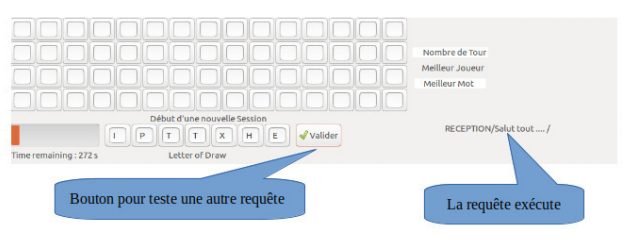
\includegraphics[width=1\textwidth]{images/1.png}
    
\subsection{ L’interface Graphique }

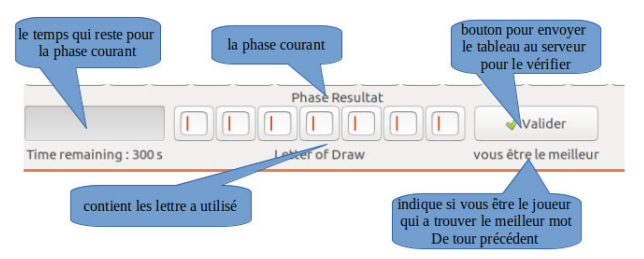
\includegraphics[width=1\textwidth]{images/2.png}
    
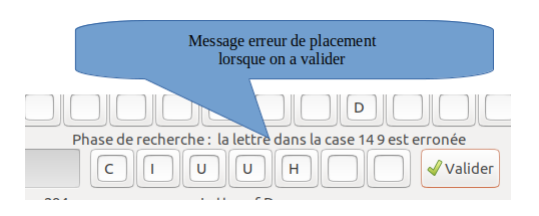
\includegraphics[width=1\textwidth]{images/3.png}
    
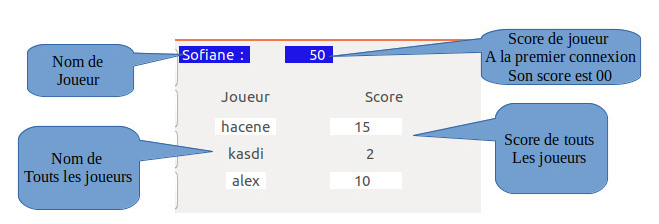
\includegraphics[width=1\textwidth]{images/4.png}
    
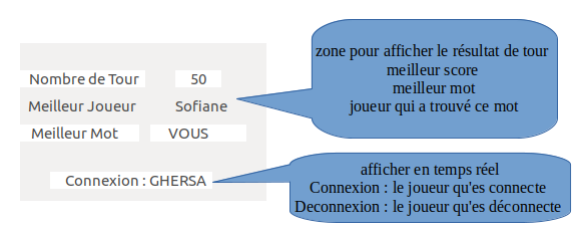
\includegraphics[width=1\textwidth]{images/5.png}
    
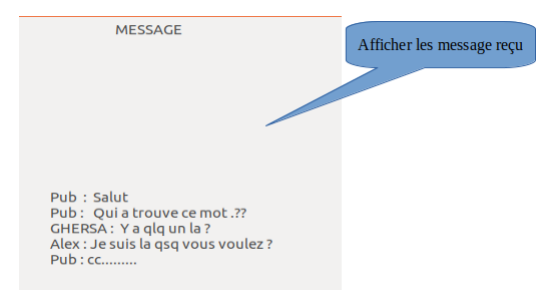
\includegraphics[width=1\textwidth]{images/6.png}
    
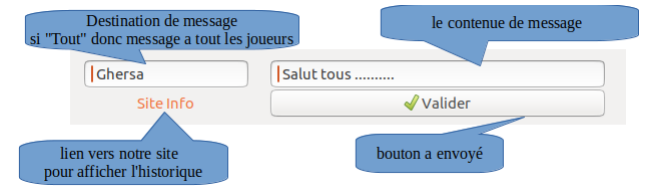
\includegraphics[width=1\textwidth]{images/7.png}
    


\end{document}